\documentclass[3p,times,procedia]{elsarticle}
\flushbottom

\usepackage{ecrc}
\usepackage[bookmarks=false]{hyperref}
\hypersetup{colorlinks,linkcolor=blue,citecolor=blue,urlcolor=blue}
\urlstyle{same}   % URLs in the text font (shorter reference list)

\usepackage{amssymb}
\usepackage{amsmath}   % needed only for \text{} in the learning-rate symbol
\usepackage{xcolor}
%% Only for XeLaTeX/Tectonic builds: txfonts (Times) has no Unicode-encoded text
%% fonts, so use the TeX Gyre Times clone instead. pdfLaTeX builds (Overleaf) are
%% unaffected and keep the template's Times fonts.
\usepackage{iftex}
\ifXeTeX
  \usepackage{fontspec}
  \setmainfont{texgyretermes}[Extension=.otf, UprightFont=*-regular,
    BoldFont=*-bold, ItalicFont=*-italic, BoldItalicFont=*-bolditalic]
  \setsansfont{texgyreheros}[Extension=.otf, UprightFont=*-regular,
    BoldFont=*-bold, ItalicFont=*-italic, BoldItalicFont=*-bolditalic]
  \setmonofont{texgyrecursor}[Extension=.otf, UprightFont=*-regular,
    BoldFont=*-bold, ItalicFont=*-italic, BoldItalicFont=*-bolditalic]
\fi

%% ---------------------------------------------------------------------------
%% Revision marking: only text that is new or changed relative to the original
%% submission is highlighted in yellow (\rev{...}); table bodies and figures are
%% not highlighted, only the changed parts of their captions.
%%  * LuaLaTeX (recommended; Overleaf: Menu > Compiler > LuaLaTeX): uses hl.lua,
%%    which must sit next to this file.
%%  * pdfLaTeX: falls back to the soul package (\hl).
%% For the clean camera-ready version change \showrevtrue to \showrevfalse.
%% ---------------------------------------------------------------------------
\usepackage{array}
\definecolor{revhl}{RGB}{255,246,140}
\newif\ifshowrev
\showrevfalse
\ifshowrev
  \ifLuaTeX
    \directlua{dofile("hl.lua")}
    \DeclareRobustCommand{\rev}[1]{{\hlattr=1 #1}}
    \makeatletter\let\EP@outputpage\@outputpage
    \def\@outputpage{\unsetattribute\hlattr\EP@outputpage}\makeatother
  \else
    \usepackage{soul}
    \sethlcolor{revhl}
    \soulregister{\cite}{7}\soulregister{\ref}{7}\soulregister{\emph}{1}\soulregister{\texttt}{1}
    \DeclareRobustCommand{\rev}[1]{\hl{#1}}
  \fi
\else
  \DeclareRobustCommand{\rev}[1]{#1}
\fi

%% Float placement tuning so figures/tables stay near their reference
\renewcommand{\topfraction}{0.92}
\renewcommand{\bottomfraction}{0.85}
\renewcommand{\textfraction}{0.06}
\renewcommand{\floatpagefraction}{0.80}
\setcounter{topnumber}{3}
\setcounter{bottomnumber}{2}
\setcounter{totalnumber}{5}

\graphicspath{{./}}
\DeclareGraphicsExtensions{.pdf,.png,.jpeg,.jpg}

%% ---------------------------------------------------------------------------
%% Camera-ready formatting (ICMLDE 2026 instructions)
%% ---------------------------------------------------------------------------
\makeatletter
%% (vi) "Keywords:" label at 8 pt like the keywords themselves (ecrc: 9 pt);
%% otherwise identical to the definition in ecrc.sty.
\def\keyword{%
\vskip0.5pt
  \def\sep{\unskip; }%
 \def\MSC{\@ifnextchar[{\@MSC}{\@MSC[2000]}}
  \def\@MSC[##1]{\par\leavevmode\hbox {\it ##1~MSC:\space}}%
  \def\PACS{\par\leavevmode\hbox {\it PACS:\space}}%
  \def\JEL{\par\leavevmode\hbox {\it JEL:\space}}%
  \global\setbox\keybox=\vbox\bgroup\hsize=\textwidth
  \normalsize\normalfont\def\baselinestretch{1}
  \parskip\z@
  \elsarticle@keyfont\noindent{\fontsize{8}{10}\selectfont\itshape Keywords: }
  \raggedright                         % Keywords are not justified.
  \ignorespaces}
%% (viii) Centre figure captions that run over one line as well (ecrc only
%% centres one-line ones); table captions stay left-aligned. Otherwise
%% identical to the definition in ecrc.sty.
\long\def\@makecaption#1#2{%
\vspace*{-3.7pt}
  \vskip\abovecaptionskip\footnotesize
  \sbox\@tempboxa{#1. #2}%
  \ifdim \wd\@tempboxa >\hsize
    \ifx\FigName\@captype
      {\centering #1. #2\par}%
    \else
      #1. #2\par
    \fi
  \else
    \global \@minipagefalse
    \ifx\FigName\@captype%
    \hb@xt@\hsize{\hfil\box\@tempboxa\hfil}%
    \else
    \hb@xt@\hsize{\box\@tempboxa}%
    \fi
  \fi
  \vskip\belowcaptionskip}
\makeatother
%% (xiii) Sort and compress citation numbers, e.g. [22-39]
\biboptions{sort&compress}

%% Running-head / logo configuration required by ecrc
\volume{00}
\firstpage{1}
\journalname{Procedia Computer Science}
\runauth{S. Salot et al.}
\jid{procs}

\begin{document}
\begin{frontmatter}

\dochead{5th International Conference on Machine Learning and Data Engineering}

\title{EchoPath: A Real-Time Assistive Indoor Navigation System For The
Visually Impaired Using Computer Vision}

\author[a]{Sakshi Salot}
\author[a]{Harsh Raj}
\author[a]{Vedant Jadhav}
\author[a]{Pratima Chauhan}
\author[a]{Sachin Bansal}
\author[a]{Vipul~Kumar~Mishra}
\author[a]{Shweta Saharan\corref{cor1}}

\address[a]{Department of Artificial Intelligence and Data Science, Gati Shakti
Vishwavidyalaya, Vadodara, Gujarat 390004, India}

\begin{abstract}
People with visual impairments face significant challenges when navigating
complex indoor environments independently. India has over 35~million
visually impaired individuals, many of them of college-going age, and
successive All India Survey on Higher Education (AISHE) reports record a
steep decline in the number of enrolled students with disabilities between
2019 and 2022. This paper proposes EchoPath, an infrastructure-free
assistive navigation system that combines a fine-tuned YOLOv8n detector,
\rev{trained on a 17-class indoor dataset assembled from COCO 2017 and
public Roboflow Universe datasets}, with MiDaS Small depth estimation and a
priority-based text-to-speech (TTS) alert pipeline. We report the
submitted model (Training~v3, mAP@50 of 0.869 on its own validation split)
and a revised model (Training~v4), retrained because the v3 classes were
strongly imbalanced, on a rebuilt dataset with importance-weighted class
balancing, attributed sources, no training--validation leakage and completed
labels. \rev{On identical leakage-free validation images, v4 raises the mean
mAP@50 over the 17 classes from 0.608 to 0.813}, and recall at the deployment
threshold for stairs from 0.25 to 0.87, waste bins from 0.08 to 0.95 and
elevators from 0.63 to 0.96. \rev{On an RTX~4500 Ada GPU the full pipeline
processes 13.9 frames per second, with a median of 0.62~s from frame capture
to the start of speech.} \rev{In 13 recorded walkthroughs, 77\% of spoken alerts
are correct, but 57\% of the obstacles in the walking path are not
announced}, mostly because they are not detected. YOLOv8n runs 3.7 times
faster than RT-DETR-L with a tenth of its weights, while RT-DETR-L is more
accurate before fine-tuning.
\end{abstract}

\begin{keyword}
Object detection \sep YOLOv8 \sep Assistive technology \sep Visual
impairment \sep Audio navigation \sep Real-time detection \sep Indoor
navigation \sep Text-to-speech \sep Monocular depth estimation
\end{keyword}

\cortext[cor1]{Corresponding author.}
\end{frontmatter}
\email{shweta.saharan@gsv.ac.in}

\vspace*{-6pt}

\section{Introduction}
\label{sec:intro}

According to the World Health Organization, 2.2 billion people have some
level of visual impairment~\cite{who2023}. India has approximately
4.95~million blind people and an estimated 35~million with some degree of
visual impairment, including about 0.24~million blind children, and the
majority of people with visual impairment are between 18 and 24 years old,
the typical age for entering college~\cite{singh2022}. Yet of approximately
92,000 students with an identified disability enrolled in Indian
colleges~\cite{aishe2021}, only an estimated 25,000 to 35,000 are visually
impaired~\cite{aishe2019,aishe_impaired_data}. Mobility and orientation are
among the most common challenges of these students, many of whom depend on
classmates to move around campus~\cite{at2030}, and independent campus
navigation was identified as a primary barrier to higher education at
Aligarh Muslim University~\cite{abdul2023}. Object detection has advanced
considerably with the YOLO family~\cite{redmon2016yolo}; YOLOv8n, in the
Ultralytics library~\cite{jocher2023yolov8}, offers a favourable trade-off
between accuracy and computational cost.

EchoPath runs on a GPU workstation, with the NVIDIA Jetson Nano as the
planned deployment platform, and delivers guidance through a TTS interface
driven by a fine-tuned YOLOv8n detector. \rev{Four training runs were
performed: v1 (26-class output head, 24 classes with validation labels), v2
and v3 (19-class head, 17 evaluated classes; v3 is the submitted model)} and
v4, the revised 17-class model, retrained on an audited and rebalanced
dataset because the v3 classes were strongly imbalanced. The objectives
are (1)~four iterative YOLOv8n fine-tuning sessions with a per-class
analysis; (2)~a comparison of YOLOv8n with RT-DETR~\cite{zhao2023rtdetr}
across deployment metrics; (3)~a data audit (source attribution,
removal of training--validation near-duplicates, importance-weighted class
balancing) and its measured effect on per-class detection; and (4)~an
end-to-end architecture integrating detection, depth and speech.

\emph{Related work.} Early ultrasonic and infrared aids~\cite{bhatlawande2014}
offered little semantic detail indoors. YOLO-based detection reached an
average accuracy of 91.7\% over nine obstacle types in a navigation
prototype for visually impaired users~\cite{li2020yolo}, whereas
RT-DETR~\cite{zhao2023rtdetr} offers high mean average precision (mAP) at a
much higher computational cost, and monocular depth models such as
MiDaS generalise to unseen datasets without fine-tuning~\cite{ranftl2020midas}.
NavCog's Bluetooth beacons reduce cognitive load but require
installation~\cite{ahmetovic2016navcog}, and non-speech spatial sounds can
outperform verbal commands~\cite{ahmetovic2019sonification}. Camera-based
systems are accurate but often too demanding for economical
devices~\cite{messaoudi2022}; VISA~\cite{yu2025visa} combined indoor
positioning, object detection and text recognition in a far more complex
system. In India, MAVI~\cite{kedia2017mavi} supports outdoor mobility (RGB
camera, GPS, IMU) without indoor directional guidance, Kasture
et~al.~\cite{kasture2021} used YOLOv3 for auditory object descriptions
without directions, and Sharma et~al.~\cite{sharma2020} built ultrasonic
sidewalk devices. Little work targets academic buildings, with notice
boards, whiteboards, water dispensers and elevator panels. Unlike Microsoft
Seeing AI and Google Lookout, which lack continuous navigation and
directional guidance, EchoPath needs no infrastructure (no beacons or prior
building configuration), fuses detection with depth estimation, gives cues
for three zones (left, ahead, right) and speaks only when necessary to limit
cognitive load.

\section{Methodology}
\label{sec:method}

\subsection{System architecture}

EchoPath has three stages (Fig.~\ref{fig:pipeline}). Stage~1 captures
video at 30~frames per second; the 13 evaluation videos were recorded
with a smartphone at chest height at $1080 \times 1920$ pixels (portrait;
one at $480 \times 864$), which YOLOv8n resizes to 640~pixels internally;
deployment will use a chest-mounted camera. Stage~2 runs the fine-tuned
YOLOv8n~\cite{jocher2023yolov8} and MiDaS Small~\cite{ranftl2020midas} on
each processed frame, and Stage~3 speaks the class, zone and direction of a
detection through earphones, \rev{0.62~s after frame capture in the median
and 3.6~s at the 95th percentile} (Section~\ref{sec:latency}).

\emph{Relative depth.} \rev{EchoPath uses relative depth, not distance in metres:
MiDaS predicts relative inverse depth, defined only up to an unknown scale
and shift, and no calibration against measured distances is performed.} Each
depth map is rescaled per frame to $[0,1]$, 1 being the nearest point of the
frame (Fig.~\ref{fig:reldepth}). The median of the inner 50\% of each
detected box (clipped to the frame) is compared with the frame's 75th and
50th percentiles: above the 75th the object is \emph{close}, above the 50th
\emph{medium}, otherwise \emph{far}. \rev{``Close'' therefore means nearer than
three quarters of the visible scene, so the same object at the same distance
can fall into different zones in different scenes.} The direction is taken
from the box centre, split at one and two thirds of the frame width. \rev{No
filter restricts alerts to the walking path: any close or medium object on
the left, ahead or right can produce an alert}, and its side is spoken so
that the user can judge whether it is in the way (path-aware alternatives
are compared in Section~\ref{sec:depth}).

\begin{figure}[!t]
\centering
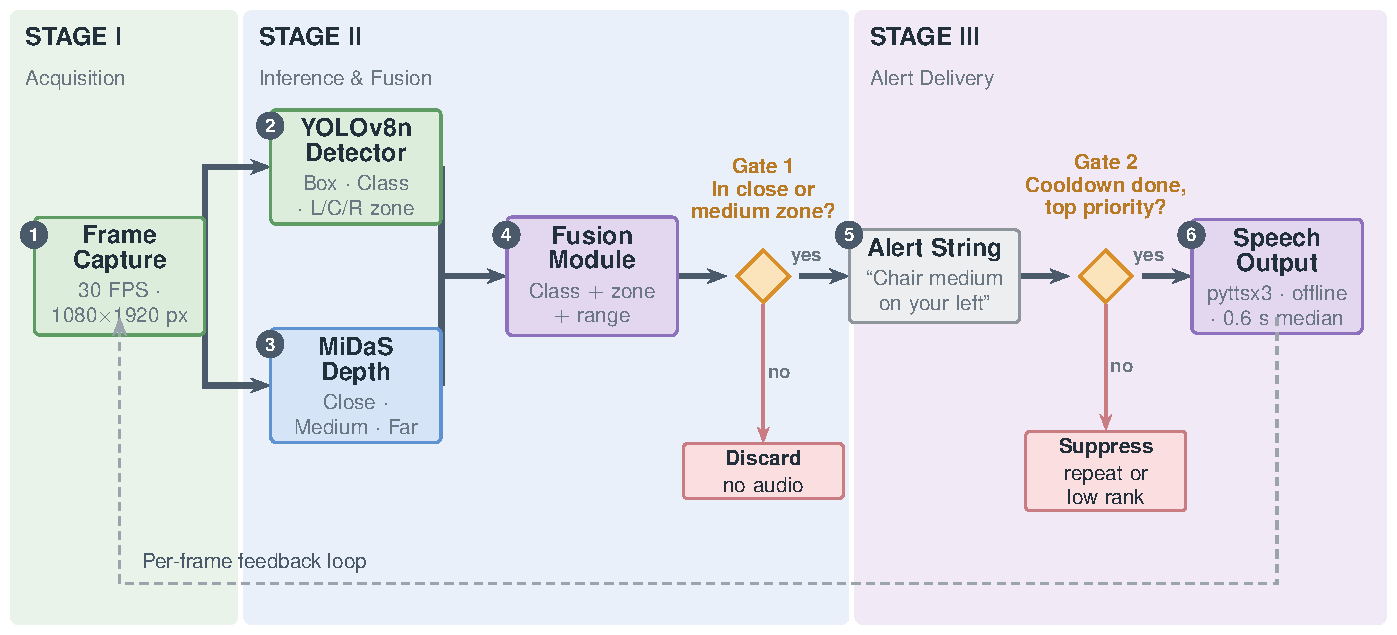
\includegraphics[width=0.62\textwidth]{fig1_new}
\caption{Architecture of EchoPath: (1)~frame capture; (2,~3)~YOLOv8n
detection and MiDaS Small depth estimation; (4)~fusion into class, lateral
zone and proximity; (5)~alert string; (6)~offline speech. Gate~1 discards
objects outside the close and medium zones and Gate~2 alerts within the
cooldown or outranked by a nearer obstacle; the dashed line is the
per-frame loop.}
\label{fig:pipeline}
\end{figure}

\subsection{Audio output module}
\label{sec:audio}

Alerts are spoken offline with pyttsx3 and state the object, zone
and side (e.g.\ ``chair close on your right''); far objects are only drawn
on the output frame. Because a phrase takes about 2.3~s, a
producer--consumer design keeps detection running: the main thread queues
alerts and a consumer thread speaks them. \rev{The consumer creates a new
engine per phrase, because a reused SAPI5 engine silently skips every phrase
after its first; this adds about 0.1~s.} \rev{In each processed frame one
candidate is considered} (a close object if any, otherwise a medium one; the
most confident within a zone), and a new alert is raised only when its
description (class, zone, direction) changes. \rev{The speaker drops an alert
within 1.5~s of the previous spoken one and does not repeat a phrase within
5~s} (the voiced evaluation videos use a 2~s gap). These limits follow
findings that repeated notifications overload a moving
user~\cite{ahmetovic2019sonification}. The audio layer only receives labels,
zones and directions, so it can be replaced (e.g.\ by haptics) without
changing detection or depth.

\subsection{Model selection: YOLOv8n versus RT-DETR}

Four deployment constraints were set: throughput above 25~FPS, model size
below 10~MB, latency below 50~ms per frame, and accuracy on safety-critical
indoor classes.
\rev{The original comparison timed the stock models on one video in a loop that
also drew and displayed every frame.} It was repeated under one setup
(Table~\ref{tab:model_compare}) for stock COCO-pretrained YOLOv8n and
RT-DETR-L~\cite{zhao2023rtdetr} (the weights used originally) and the
fine-tuned EchoPath YOLOv8n: \rev{NVIDIA RTX~4500 Ada, Ultralytics~8.4.37,
PyTorch~2.4.1+cu118 (CUDA~11.8), 640-pixel input, batch size~1, FP32} (FP16
gave no speed-up), confidence 0.40, the same 390 pre-decoded frames of the
13 videos after 50 warm-up predictions, GPU synchronised around every call,
two alternating rounds. \rev{Accuracy is the mAP@50 on the v4 validation split
for the five classes COCO shares with EchoPath} (person, chair, potted plant,
table, monitor). YOLOv8n meets all four constraints; \rev{RT-DETR-L fails only
the size constraint, not three of four as originally stated}, and is the more
accurate detector before fine-tuning. YOLOv8n was chosen because it needs a
tenth of the weights and a twelfth of the computation and runs 3.7 times
faster, which matters most on the planned Jetson Nano (not measured here),
in line with the priority of efficient methods on low-cost edge
devices~\cite{messaoudi2022}. Fine-tuning raises YOLOv8n's mAP@50 on the
shared classes to 0.575; \rev{RT-DETR-L was not fine-tuned, so whether its
advantage would persist is not known.}

\begin{table}[!t]
\caption{\rev{YOLOv8n versus RT-DETR-L under the setup of Section~2.3} (median /
95th percentile over 390 frames). Accuracy on the five classes shared with
COCO (v4 validation split); the COCO models are not fine-tuned.}
\label{tab:model_compare}
\footnotesize
\begin{tabular*}{\hsize}{@{\extracolsep{\fill}}lccc@{}}
\toprule
Metric & YOLOv8n (COCO) & RT-DETR-L (COCO) & YOLOv8n (EchoPath v4) \\
\colrule
Weights (MB) / parameters (millions) & \rev{6.5 / 3.2} & \rev{66.5 / 32.1} & \rev{6.3 / 3.0} \\
Computation (GFLOPs)                 & \rev{8.7}        & \rev{103.8}       & \rev{8.1} \\
Time per frame (ms), of which network inference & \rev{8.1 / 14.2, 5.4} & \rev{29.6 / 46.4, 26.2} & \rev{7.6 / 10.7, 5.4} \\
Frames per second                    & \rev{123}        & \rev{34}          & \rev{131} \\
mAP@50 / mAP@50-95, 5 shared classes & \rev{0.355 / 0.222} & \rev{0.410 / 0.272} & \rev{0.575 / 0.376} \\
\botrule
\end{tabular*}
\end{table}

\subsection{Dataset construction and object classes}
\label{sec:dataset}

\emph{Sources.} \rev{No training images were captured by the authors.} All come
from COCO 2017~\cite{lin2014coco} (CC~BY~4.0 annotations; each image keeps
its Flickr licence) and 18 Roboflow Universe datasets under
CC~BY~4.0~\cite{rf_person,rf_chair,rf_door,rf_navigation,rf_whiteboard,rf_notice,rf_elevatordoor,rf_column,rf_window,rf_water,rf_plant,rf_wastebin,rf_dustbin,rf_trashbin,rf_fire,rf_wetfloor,rf_table,rf_monitor},
\rev{each supplying one or two classes;} \rev{Supplementary Table~S1 lists the author,
URL, version, licence, classes, image counts and our changes} (remapped
names, dropped classes, merges) of every source. The 17 classes are listed
by tier in Section~\ref{sec:training}. \rev{The 13 evaluation videos, recorded by
the authors in the Academic Block Building, contain no training images.}

\emph{Splits (Table~\ref{tab:datasets}).} \rev{Every version kept each source's
predefined split (COCO train2017 to training, val2017 to validation)};
\rev{nothing was re-split, and frames of one source video were not grouped.}
\rev{Backpack (1,238 v3 training labels) and handbag (6) had no validation labels
in v1 to v3}, hence the evaluated classes in Table~\ref{tab:datasets}. In v1
and v2 the sources' test images formed a test split; \rev{from v3 on they were
merged into training} (v3: 36,765 training labels). \rev{A test split was not
needed because (1)~no hyperparameter was tuned on the validation split}
(Section~\ref{sec:training}); (2)~the validation split only selects the best
epoch, and the best and final epochs differ by at most 0.0014 in mAP@50 in
any run (they coincide for v1 and v3), so validation results are effectively
held-out results; and (3)~a test split from the same public sources would
measure the same distribution, whereas the relevant test is footage from the
target building, which no source contains: the 13 videos, whose annotation
as a labelled test set is planned (Section~\ref{sec:discussion}).

\emph{Audit of v3.} \rev{(i)~Leakage: 25.6\% of v3 validation images have a
near-duplicate in training} (difference hash, Hamming distance $\leq 4$;
8.4\% identical), mostly consecutive video frames that the sources placed in
both splits, concentrated in person (87\% of validation labels),
water\_dispenser (93\%), slide (56\%), whiteboard (51\%) and notice\_board
(47\%); the archived v1 and v2 datasets give 42.8\% and at most 26.6\%, so
leakage inflated the validation results of v1 to v3. (ii)~The sources of
the stairs, elevator, potted\_plant and monitor data could not be
identified. (iii)~The 769 COCO chair images carried only chair labels,
although COCO annotates 2,364 people, 463 dining tables, 197 potted plants
and 108 televisions in them, which the model learned as background.
\rev{(iv)~The class counts were mislabelled in the original submission: the
largest v3 class is fire\_extinguisher, not column} (Fig.~\ref{fig:labels}a).

\emph{Why v4 was retrained.} \rev{The v3 classes were strongly imbalanced
(10,929 fire\_extinguisher against 106 waste\_bin labels, 103:1)}, reflecting
the sizes of the merged datasets, inflated by pre-augmented copies in some
sources, rather than each class's importance for navigation. The v4 training split is therefore balanced by importance
(Section~\ref{sec:training}), and the rebuild also fixed the other findings:
(1)~\rev{the four unattributable sources and the backpack/handbag source were
removed (17 classes)}; (2)~real-world data were added for stairs and
elevator~\cite{rf_navigation,rf_elevatordoor}, monitor~\cite{rf_monitor},
potted plant~\cite{rf_plant} and waste bin~\cite{rf_dustbin,rf_trashbin},
plus 311 indoor COCO potted-plant images licensed CC~BY~2.0, ``no known
copyright restrictions'' or United States Government work; six visually
inspected candidates were rejected (floor plans, toy miniature scenes,
catalogue and watermarked stock photographs, printed elevator pictures,
strong fisheye distortion); (3)~COCO's person, chair, potted plant, dining
table and television labels were added to every COCO image; and (4)~\rev{all
2,727 training images within Hamming distance~4 of a validation image were
removed, leaving the validation split unchanged} \rev{(v4: 33,539 training and
5,863 validation labels)}.

\begin{table}[!t]
\caption{\rev{Dataset versions and results on each run's own validation split.}
``Head'' is the number of output classes, ``eval.'' the number with
validation labels; leakage is the share of validation images with a
near-duplicate (Hamming distance $\leq 4$) in training. v2's data are
reconstructed from an archived copy made before table and monitor were added
(21,601 / 2,352 / 1,211 images) plus the table and monitor images identified
in v3: validation is exact, training and test sizes are derived from the
logged batches per epoch, and leakage is an upper bound. Absolute changes:
v1 to v2 $+$0.068 P, $+$0.134 R, $+$0.107 mAP@50, $+$0.108 mAP@50-95; v2 to
v3 $-$0.014, $-$0.040, $-$0.039 ($-$4.3\% relative) and $-$0.042.}
\label{tab:datasets}
\footnotesize
\setlength{\tabcolsep}{3pt}
\begin{tabular*}{\hsize}{@{\extracolsep{\fill}}lcccccccc>{\raggedright\arraybackslash}p{2.75cm}@{}}
\toprule
Version & Head / eval. & Train & Val. & Test & Val.\ labels & Leakage & P / R & mAP@50 / 50-95 & Purpose of the run \\
\colrule
v1 & \rev{26 / 24} & \rev{23,445} & \rev{2,865} & \rev{1,367} & \rev{5,046} & \rev{42.8\%} & \rev{0.833 / 0.727} & \rev{0.801 / 0.633} & \rev{Baseline} \\
v2 & \rev{19 / 17} & \rev{$\approx$23,700} & \rev{2,580} & \rev{$\approx$1,340} & \rev{4,453} & \rev{$\leq$26.6\%} & 0.901 / 0.861 & 0.908 / 0.741 & \rev{Fewer classes, new sources} \\
v3 (submitted) & \rev{19 / 17} & \rev{25,666} & \rev{2,780} & -- & \rev{5,017} & \rev{25.6\%} & 0.887 / 0.821 & 0.869 / 0.699 & \rev{Adds 800 COCO chair images} \\
v4 (revised) & \rev{17 / 17} & \rev{20,307} & \rev{2,922} & -- & \rev{5,863} & \rev{0\% (removed)} & \rev{0.855 / 0.787} & \rev{0.828 / 0.664} & \rev{Rebalanced, audited data} \\
\botrule
\end{tabular*}
\end{table}

\begin{figure}[!t]
\centering
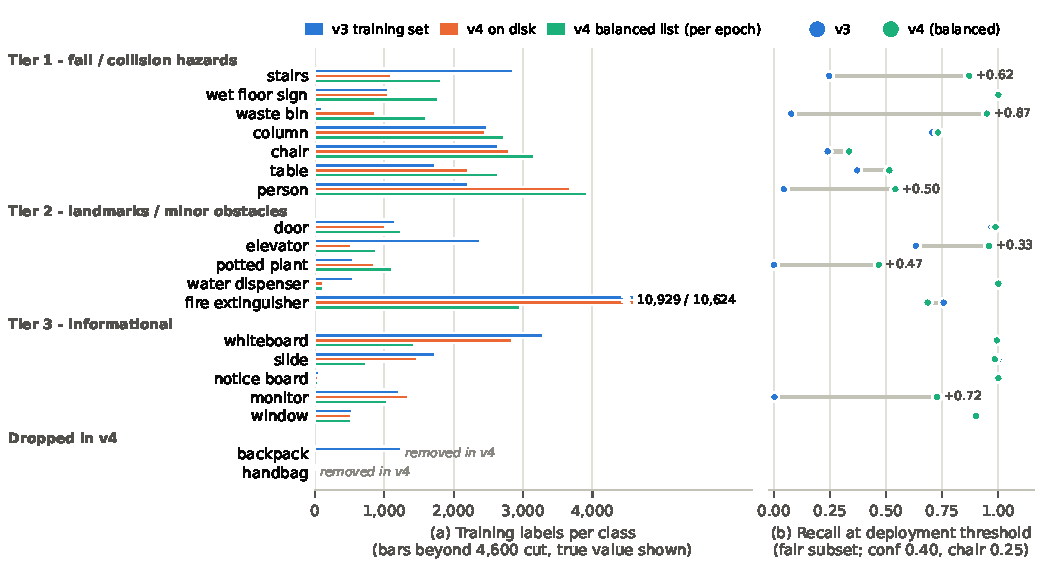
\includegraphics[width=0.68\textwidth]{labels_recall_v3_v4}
\caption{\rev{(a)~Training labels per class for v3 and v4}, by importance tier
(Section~\ref{sec:training}); \rev{the v3 imbalance is why v4 was retrained}, and
the v4 balanced list is what v4 sees per epoch. (b)~Recall at the deployment threshold (confidence
0.40; chair 0.25) of v3 and v4 on the fair validation subset (no
near-duplicate in either training split); changes $\geq 0.3$ are printed.}
\label{fig:labels}
\end{figure}

\subsection{Training configuration and hyperparameter tuning}
\label{sec:training}

All runs fine-tuned COCO-pretrained YOLOv8n~\cite{jocher2023yolov8} for
100~epochs at $640 \times 640$ with batch size 64 (Ultralytics~8.4.37,
PyTorch~2.4.1+cu118, NVIDIA RTX~4500 Ada, 24~GB). The automatic optimiser
selected MuSGD (momentum 0.9, weight decay 0.0005); after a three-epoch
warm-up the learning rate of the first parameter group peaked at 0.03 (three
times the base rate of 0.01 of the other groups) and decayed linearly to
0.0006. Augmentation was identical in every run: mosaic ($p=1.0$, off for
the last 10 epochs), horizontal flips ($p=0.5$), HSV jitter (0.015, 0.7,
0.4), translation 0.1 and scaling 0.5; \rev{no mixup or copy-paste was used in
any run, contrary to the original statement for v3}. v2 and v3 therefore
differ only in their data (v3 adds 800 COCO chair images, 600 for training
and 200 for validation, and merges v2's test images into training); the
v1-to-v2 gain coincides with the reduction from 26 to 19 classes and the
revised sources and, as the validation splits differ, cannot be attributed
to a single factor.

\emph{\rev{Importance-weighted class balancing (v4 training split only).}} Tier~1
holds fall and collision hazards (stairs, wet\_floor\_sign, waste\_bin,
column, chair, table, person), tier~2 landmarks and minor obstacles (door,
elevator, potted\_plant, water\_dispenser, fire\_extinguisher) and tier~3
informational classes, announced like the others but least important for
safe walking (whiteboard, slide, notice\_board, monitor, window). \rev{Images
containing only over-represented, lower-importance classes were first
undersampled with a fixed seed} (fire\_extinguisher to about 3,000 labels,
monitor to about 1,000, half of the whiteboard- or slide-only images).
Repeat-factor sampling then gives each class
$r_c = \min\left(3, \sqrt{T_c / f_c}\right)$, with label count $f_c$ and
$T_c$ of 3,000 for tier~1 and 1,500 for tier~2 (tier~3 and the synthetic
water\_dispenser source are never repeated), and repeats each image by the
largest $r_c$ of its labels with stochastic rounding. The 17,110-entry list
draws on 14,022 unique images, so no image is duplicated on disk, and
random mosaic, flip and colour augmentation make each repeat look different
(Fig.~\ref{fig:labels}a, Table~\ref{tab:perclass}).

\section{Experimental results}
\label{sec:results}

\subsection{Detection results}
\label{sec:v4}

\emph{v2 and v3.} Their own-split results (Table~\ref{tab:datasets}) are
not comparable, because
v3's split adds 200 COCO chair images to v2's. \rev{On
v3's split v2 scores 0.848 and v3 0.869 (0.813 and 0.837 without validation
images that near-duplicate a training image), so v3 was the stronger model
and was retained}; \rev{v2's originally reported chair recall of 1.000 came from a
split without COCO chair scenes (0.152 versus 0.239 for v3 on the shared
split)}. \rev{Validation loss was still decreasing at epoch~100 in v1 to v3, so no
run overfitted.}
For v3, the PR curve gives an mAP@50 of 0.995 for person, whiteboard,
notice\_board and water\_dispenser, \rev{the four classes with the highest
leakage, so these scores overstate real-world performance}; precision is
1.00 at maximum confidence, recall 0.94 at confidence 0, and F1 peaks at
0.84 at confidence 0.448.

\emph{Confusion matrices.} \rev{v3's matrix (Fig.~\ref{fig:cms}a) has empty
backpack and handbag rows and columns (no validation labels), which is why
17 classes are evaluated; v4's (Fig.~\ref{fig:cms}b) has exactly 17.}
\rev{Diagonal entries are recall at Ultralytics' confusion-matrix operating point
(confidence 0.25, IoU 0.45), whereas Table~\ref{tab:perclass} gives recall at
the confidence that maximises the mean F1; hence v3's chair recall is 0.30
in the matrix but 0.241 in the table} (fire\_extinguisher 0.82 versus 0.743).
Chair is v3's weakest class: 85\% of its 665 validation labels come from
cluttered COCO scenes, where its recall is 0.24, against 1.00 on the
Roboflow chair images. The 0.43 in v3's background column means that 43\% of
its false detections on background were predicted as fire\_extinguisher; it
is not a miss rate. \rev{Recalls of 1.00 for slide, notice\_board,
water\_dispenser and wet\_floor\_sign come from small validation sets
(Table~\ref{tab:perclass}), with heavy leakage for the first three, and do
not indicate perfect real-world detection.}

\emph{v4.} v4 ran all 100 epochs (3.1~h, best epoch 94;
Table~\ref{tab:perclass}). Its own-split results are lower than v3's because
its split is harder: no validation image has a near-duplicate in training,
and the completed COCO labels add many people, tables and plants in
cluttered scenes, which lowers person, table and potted\_plant in
Table~\ref{tab:perclass}. Re-scored on the same v4 validation images, with v3's 19
outputs mapped onto the 17 classes, the mean mAP@50 rises from 0.632 to
0.827 ($+$0.195) on all 2,922 images and \rev{from 0.608 to 0.813 ($+$0.205) on a
fair subset of 2,247 images with no near-duplicate in either training split}
(mAP@50-95 from 0.522 to 0.663 and from 0.500 to 0.646), so v3's own split
(0.869) strongly favoured it. \rev{The
largest recall gains (Fig.~\ref{fig:labels}b) are for waste\_bin, monitor,
stairs, person, potted\_plant and elevator.} The gains for person, table
and chair come mainly from the completed COCO labels (v3, trained to treat
unlabelled people as background, finds only 4\% of people in crowded
scenes); those for stairs, elevator, monitor, potted\_plant and waste\_bin
partly reflect the new sources and so also measure generalisation. As data
and class balance changed together, \rev{the gains show the combined effect of
the rebuild and cannot be attributed to the balancing alone.}
\rev{Fire\_extinguisher recall falls by 0.07, a deliberate consequence of
undersampling 4,588 fire-extinguisher-only images}, and
water\_dispenser by 0.10 on the full set, because 127 of its 136 validation
images near-duplicate v3's training images (both models score 1.00 on the
nine unseen ones). \rev{For wet\_floor\_sign (43 of 43 detected) the two-sided
95\% Clopper--Pearson lower bound is 0.92, for waste\_bin (74 of 78) the
95\% Wilson interval is 0.88--0.98}, and window and notice\_board are too
small for firm conclusions.

\begin{table}[!t]
\caption{\rev{Per-class results of Training~v3 (submitted) and Training~v4
(revised, class-balanced)}, each on its own validation split; \rev{P and R at the
confidence that maximises each run's mean F1.} For v4 the table also gives
the training labels on disk and per epoch in the balanced list, the
validation labels, and \rev{P and R at the deployment threshold of 0.40}; the v3
and v4 splits differ (Section~\ref{sec:v4}).}
\label{tab:perclass}
\scriptsize
\setlength{\tabcolsep}{2.5pt}
\begin{tabular*}{\hsize}{@{\extracolsep{\fill}}lccccccccccccc@{}}
\toprule
& \multicolumn{4}{c}{Training v3 (17 cls) - Submitted}
& \multicolumn{9}{c}{Training v4 (17 cls) - Revised} \\
& & & & & \multicolumn{3}{c}{Labels} & & & & & \multicolumn{2}{c}{At 0.40} \\
Class & P & R & mAP50 & 50-95 & Train & Bal. & Val. & P & R & mAP50 & 50-95 & P & R \\
\colrule
\textbf{all} & 0.887 & 0.821 & 0.869 & 0.699 & \rev{33,539} & \rev{27,751} & \rev{5,863} & \rev{0.855} & \rev{0.787} & \rev{0.828} & \rev{0.664} & & \\
person & 0.974 & 0.990 & 0.995 & 0.815 & \rev{3,676} & \rev{3,922} & \rev{743} & \rev{0.769} & \rev{0.598} & \rev{0.694} & \rev{0.433} & \rev{0.697} & \rev{0.645} \\
chair & 0.746 & 0.241 & 0.354 & 0.260 & \rev{2,807} & \rev{3,163} & \rev{666} & \rev{0.680} & \rev{0.287} & \rev{0.388} & \rev{0.284} & \rev{0.595} & \rev{0.311} \\
door & 0.959 & 0.972 & 0.989 & 0.891 & \rev{1,016} & \rev{1,241} & \rev{292} & \rev{0.957} & \rev{0.979} & \rev{0.989} & \rev{0.892} & \rev{0.947} & \rev{0.990} \\
stairs & 0.870 & 0.792 & 0.897 & 0.723 & \rev{1,102} & \rev{1,817} & \rev{138} & \rev{0.921} & \rev{0.848} & \rev{0.912} & \rev{0.597} & \rev{0.898} & \rev{0.870} \\
slide & 0.989 & 1.000 & 0.995 & 0.983 & \rev{1,472} & \rev{736} & \rev{147} & \rev{0.970} & \rev{0.993} & \rev{0.994} & \rev{0.963} & \rev{0.969} & \rev{0.993} \\
whiteboard & 0.993 & 0.993 & 0.995 & 0.980 & \rev{2,846} & \rev{1,431} & \rev{301} & \rev{0.996} & \rev{0.990} & \rev{0.995} & \rev{0.963} & \rev{0.994} & \rev{0.990} \\
notice\_board & 0.945 & 1.000 & 0.995 & 0.995 & \rev{48} & \rev{48} & \rev{17} & \rev{0.894} & \rev{1.000} & \rev{0.995} & \rev{0.964} & \rev{0.881} & \rev{1.000} \\
elevator & 0.908 & 0.917 & 0.955 & 0.653 & \rev{524} & \rev{881} & \rev{95} & \rev{0.980} & \rev{0.937} & \rev{0.965} & \rev{0.654} & \rev{0.948} & \rev{0.958} \\
column & 0.733 & 0.663 & 0.714 & 0.495 & \rev{2,458} & \rev{2,725} & \rev{252} & \rev{0.713} & \rev{0.669} & \rev{0.720} & \rev{0.509} & \rev{0.681} & \rev{0.730} \\
window & 0.730 & 0.900 & 0.895 & 0.583 & \rev{529} & \rev{529} & \rev{10} & \rev{0.761} & \rev{0.900} & \rev{0.895} & \rev{0.624} & \rev{0.699} & \rev{0.900} \\
water\_dispenser & 0.970 & 1.000 & 0.995 & 0.958 & \rev{115} & \rev{115} & \rev{136} & \rev{0.984} & \rev{0.902} & \rev{0.958} & \rev{0.874} & \rev{0.976} & \rev{0.905} \\
potted\_plant & 0.830 & 0.520 & 0.634 & 0.292 & \rev{852} & \rev{1,119} & \rev{75} & \rev{0.491} & \rev{0.467} & \rev{0.435} & \rev{0.279} & \rev{0.450} & \rev{0.467} \\
waste\_bin & 0.791 & 0.750 & 0.828 & 0.597 & \rev{862} & \rev{1,604} & \rev{78} & \rev{0.936} & \rev{0.942} & \rev{0.982} & \rev{0.923} & \rev{0.935} & \rev{0.949} \\
fire\_extinguisher & 0.918 & 0.743 & 0.860 & 0.624 & \rev{10,624} & \rev{2,954} & \rev{2,175} & \rev{0.903} & \rev{0.649} & \rev{0.798} & \rev{0.540} & \rev{0.868} & \rev{0.694} \\
wet\_floor\_sign & 0.930 & 1.000 & 0.977 & 0.891 & \rev{1,057} & \rev{1,779} & \rev{43} & \rev{0.957} & \rev{1.000} & \rev{0.984} & \rev{0.899} & \rev{0.948} & \rev{1.000} \\
table & 0.809 & 0.791 & 0.809 & 0.580 & \rev{2,204} & \rev{2,643} & \rev{259} & \rev{0.769} & \rev{0.517} & \rev{0.579} & \rev{0.371} & \rev{0.750} & \rev{0.541} \\
monitor & 0.988 & 0.691 & 0.883 & 0.558 & \rev{1,347} & \rev{1,044} & \rev{436} & \rev{0.854} & \rev{0.700} & \rev{0.794} & \rev{0.523} & \rev{0.814} & \rev{0.727} \\
\botrule
\end{tabular*}
\end{table}

\begin{figure}[!t]
\centerline{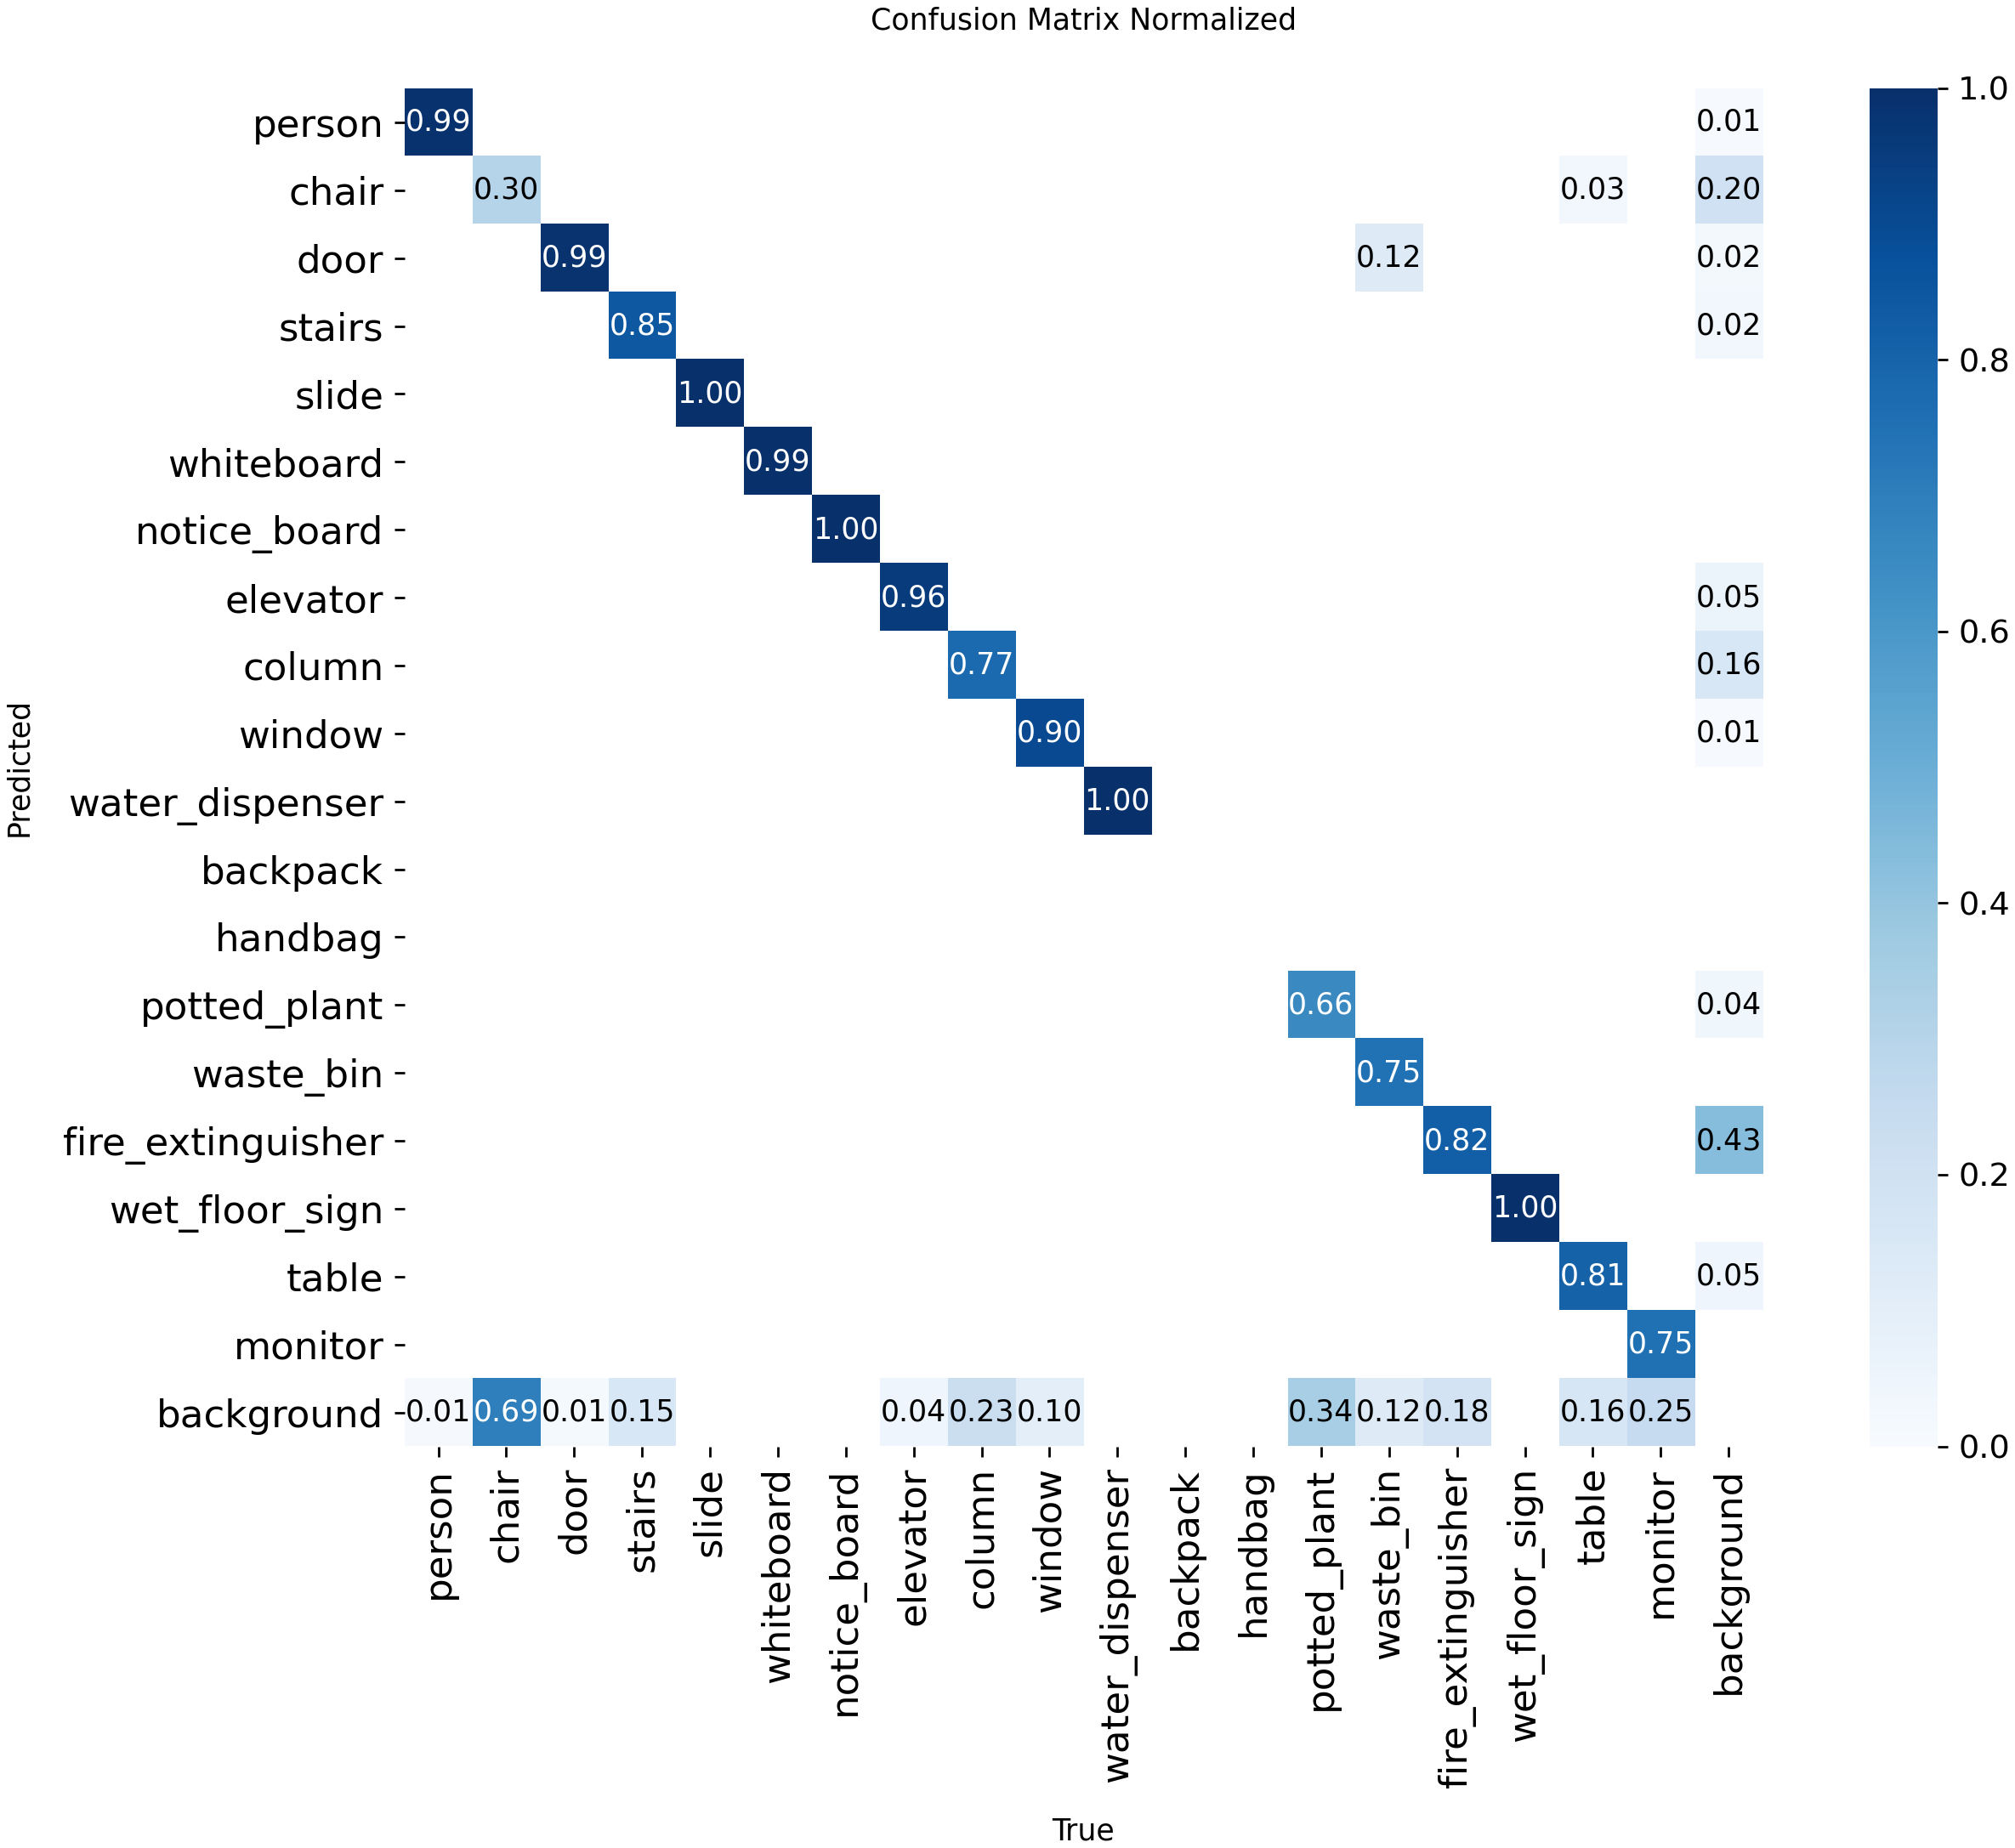
\includegraphics[width=0.39\textwidth]{cm_crop.png}\hspace*{3mm}%
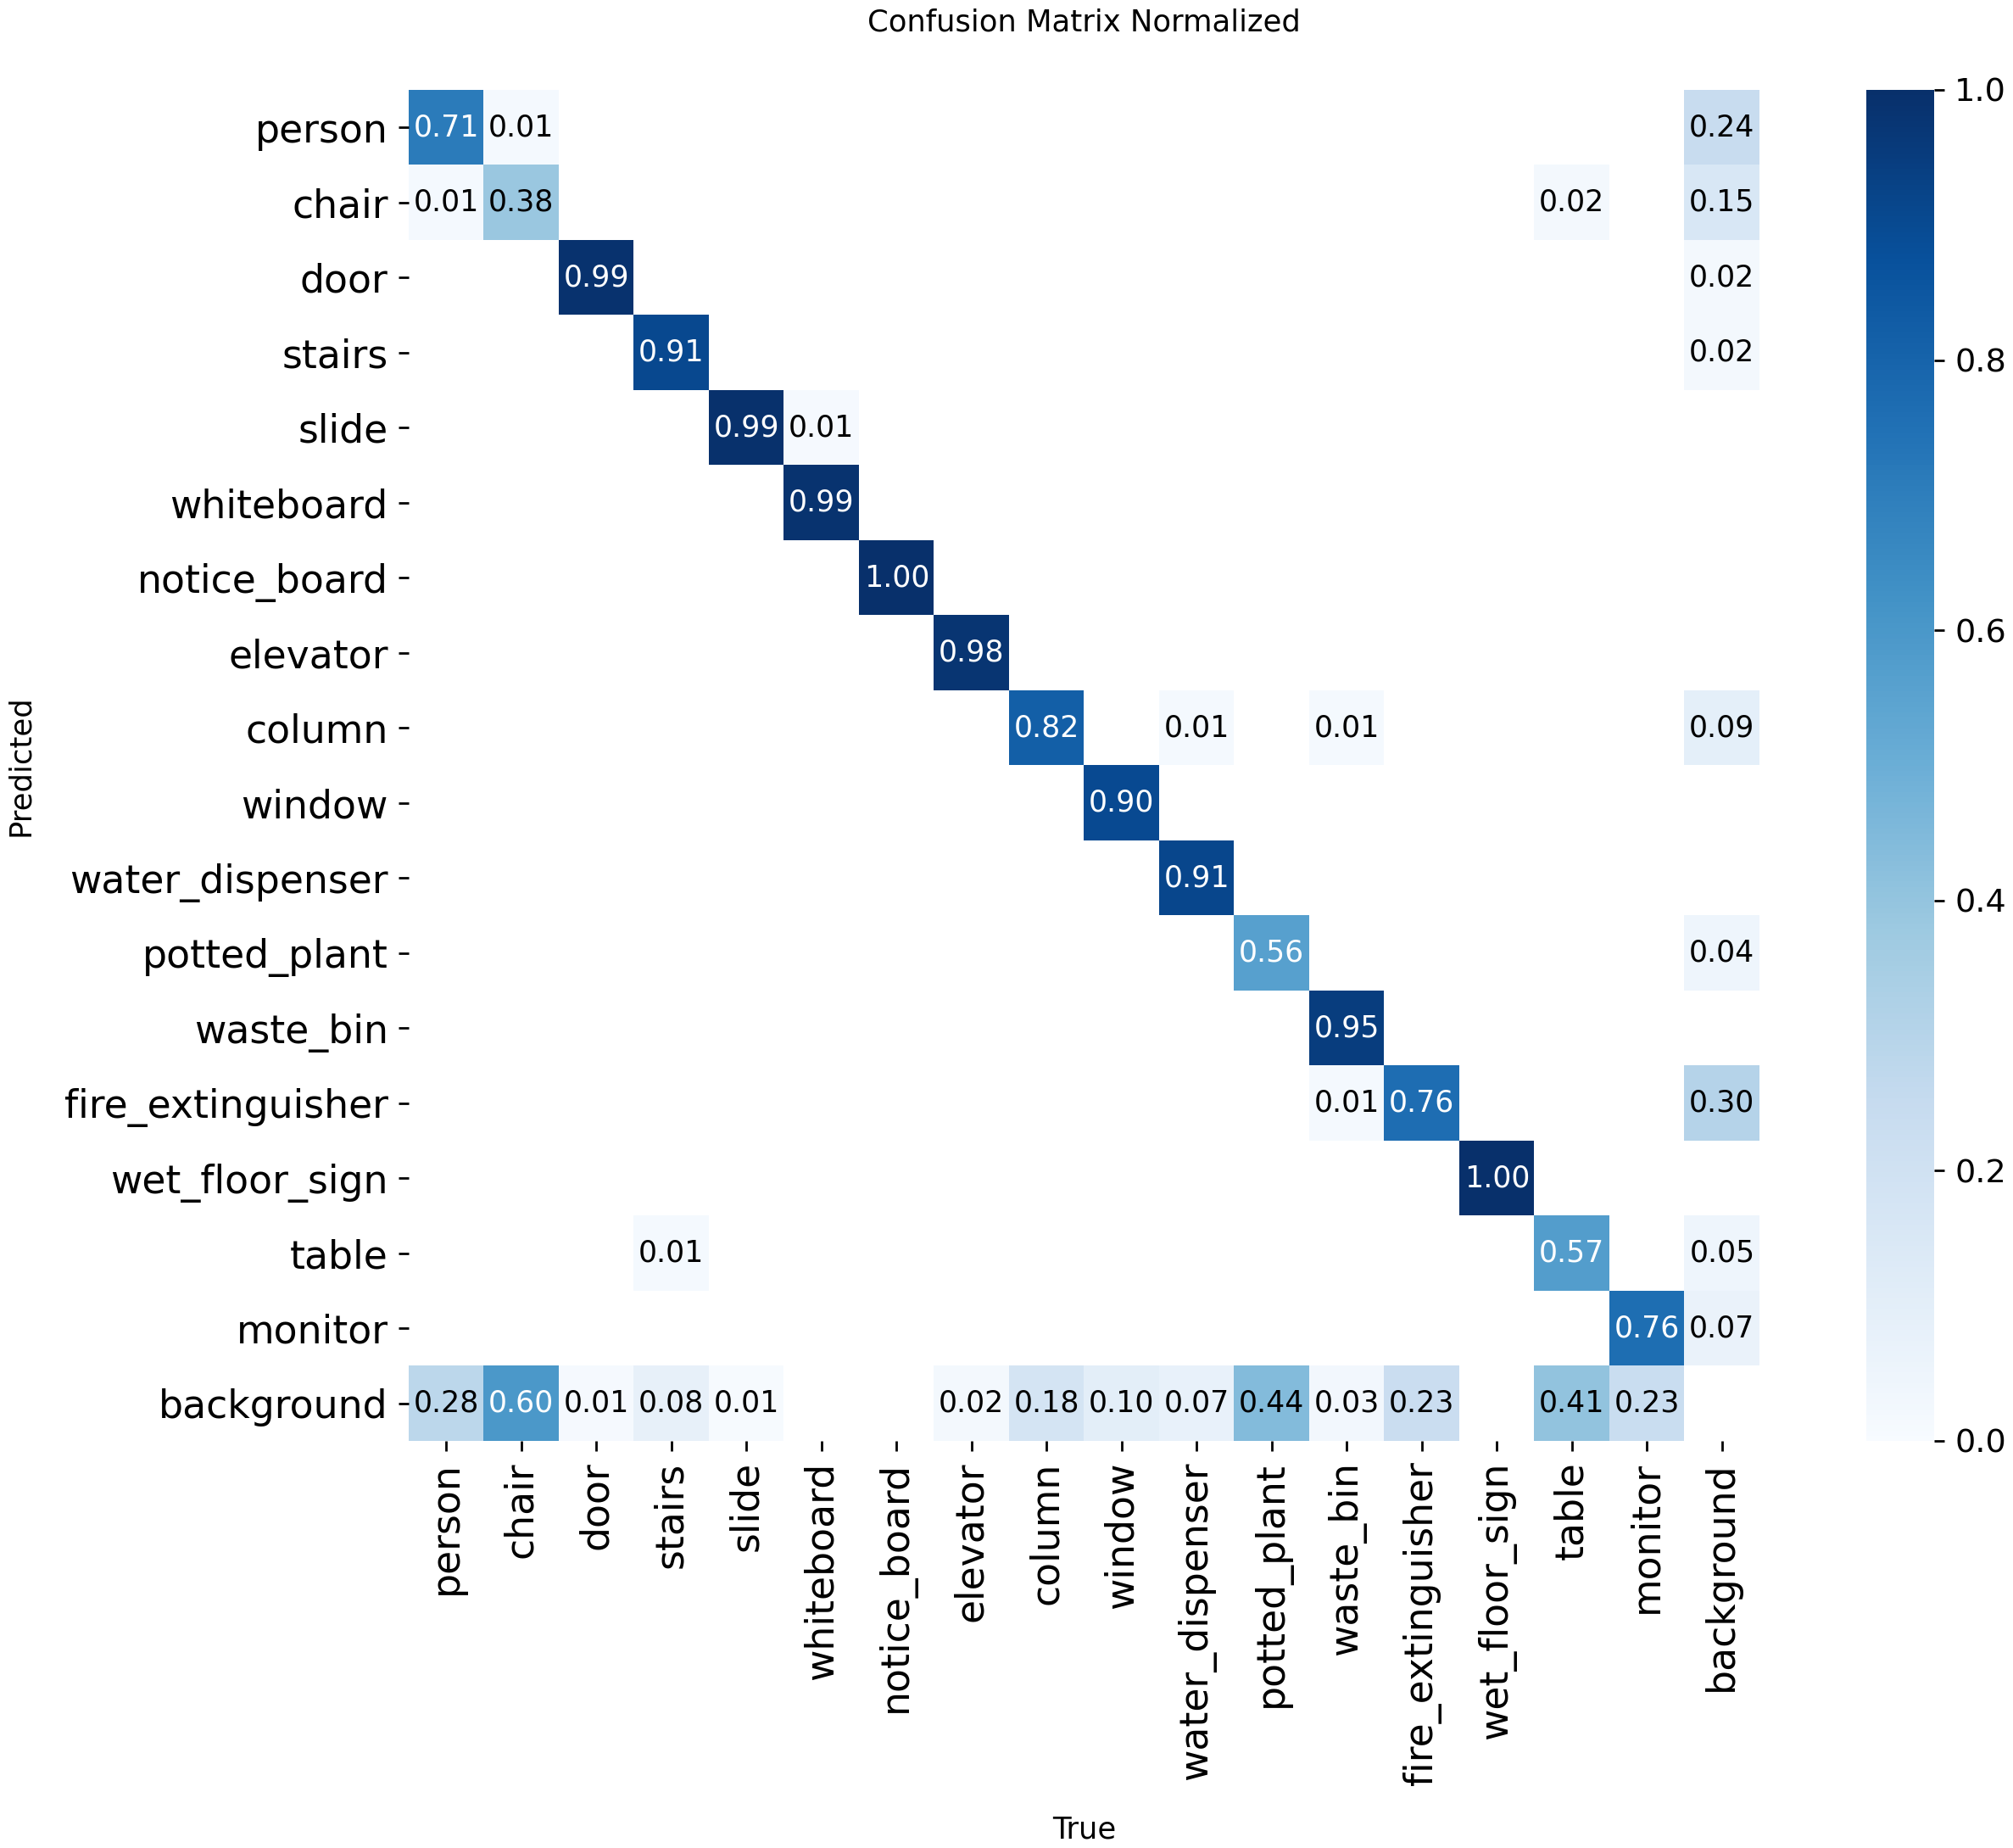
\includegraphics[width=0.39\textwidth]{cm_v4_crop.png}}
\caption{Normalised confusion matrices (confidence 0.25; diagonal entries
are per-class recall) of (a)~Training~v3, \rev{with empty backpack and
handbag rows and columns}, and \rev{(b)~Training~v4 (17 classes)}.}
\label{fig:cms}
\end{figure}

\subsection{Depth model comparison and alert quality}
\label{sec:depth}

MiDaS Small~\cite{ranftl2020midas} (torch.hub) and Depth Anything
V2 Small~\cite{depthanythingv2} (HuggingFace Transformers), both producing relative inverse depth (Fig.~\ref{fig:reldepth}), were
compared on the 13 videos. The original comparison used separate notebooks
that differed in more than the model (MiDaS: per-frame percentile
thresholds, median of the inner clipped box; Depth Anything V2: fixed
thresholds of 0.70 and 0.40, mean of the whole unclipped box; both with the
v3 detector). \rev{Both were re-run with the v4 detector in a single pass, so
that frames, detections and the alert rule are identical, under both
threshold rules} (Table~\ref{tab:depth_compare}); \rev{the deployed configuration
reproduces all 260 alerts of the pipeline exactly}. \rev{Under the same rule the
two models behave almost identically, whereas the fixed rule halves the
alerts of Depth Anything V2} (per-video counts in Supplementary Fig.~S1). The
\rev{$2.3\times$ difference reported originally (261 versus 113 alerts) therefore
came from the threshold rule and box statistic, not from the depth models},
and \rev{the claims that MiDaS has a higher false-positive tendency and that
Depth Anything V2 gives alerts more likely to match genuine hazards were
removed.}

\emph{Alert quality.} \rev{Every object of the 17 classes that comes within about
3~m of the camera was annotated in the 13 videos} with its class, side
(thirds of the frame, as in the system) and the interval during which it is
that close; objects of an obstacle class (tier~1, potted plants, water
dispensers) ahead count as hazards in the walking path (213 objects, 51
hazards). The annotations were drafted by an AI model from frames sampled at
2 per second, without access to any detector output, and then checked and
corrected by one author. \rev{An alert is correct if an annotated object of the
announced class is present within $\pm 1$~s, and a hazard is missed if no
alert names its class during its interval ($\pm 1$~s)}; proximity is not
scored, as annotated distances are visual estimates. With the deployed
configuration (Table~\ref{tab:depth_compare}, first row), \rev{77\% of spoken
alerts are correct and 82\% of these also give the correct side, but 57\%
of the hazards receive no spoken alert.} Before the 2~s gap, 35\% are missed
(0.24--0.49): 11 of the 29 missed hazards are lost to the rate limit and 18
never produce an alert, of which 14 are never detected at confidence 0.40
(e.g.~the water dispensers and waste bins of two waiting areas, bench
seats, armchairs and two flights of stairs), 3 are always placed in the far
zone and 1 was announced just before its interval. \rev{Missed hazards are
therefore mainly a detection, not a depth, problem.}

\emph{Path rule.} Of the 64 spoken alerts, 27 concern objects ahead, 21 on
the left and 16 on the right. \rev{Announcing only objects in the centre third
reduces the spoken alerts to 45 and the false alerts from 3.7 to 2.7 per
minute, with the same precision (0.76) and the same 29 of 51 missed in-path
hazards}, because the detector misses them rather than side objects crowding
them out; announcing in-path objects first and side objects only when close
does not help (54 alerts, 31 missed). \rev{Side alerts thus add to the alert load
without improving coverage of the walking path}, although they may help when
the user turns (future work~(3)).

\begin{table}[!t]
\caption{\rev{Depth model comparison with the v4 detector on the 13 videos} (same
frames and detections in every row): the deployed percentile rule
(Section~2.1) or fixed thresholds of 0.70 and 0.40, both on the inner-box
median; the last row reproduces the earlier Depth Anything V2 notebook.
\rev{Precision, false alerts and missed hazards (95\% Wilson intervals) refer to
the alerts spoken after the 2~s gap.}}
\label{tab:depth_compare}
\footnotesize
\setlength{\tabcolsep}{3pt}
\begin{tabular*}{\hsize}{@{\extracolsep{\fill}}llccccc@{}}
\toprule
Depth model & Rule & Unique alerts & Spoken & Precision & False/min & Missed hazards \\
\colrule
MiDaS Small (deployed) & \rev{percentile} & \rev{260} & \rev{64} & \rev{0.77 (0.65--0.85)} & \rev{3.7} & \rev{29/51 = 0.57 (0.43--0.69)} \\
Depth Anything V2 Small & \rev{percentile} & \rev{252} & \rev{64} & \rev{0.80 (0.68--0.88)} & \rev{3.2} & \rev{27/51 = 0.53 (0.40--0.66)} \\
MiDaS Small & \rev{fixed} & \rev{257} & \rev{61} & \rev{0.74 (0.62--0.83)} & \rev{4.0} & \rev{30/51 = 0.59 (0.45--0.71)} \\
Depth Anything V2 Small & \rev{fixed} & \rev{131} & \rev{38} & \rev{0.71 (0.55--0.83)} & \rev{2.7} & \rev{38/51 = 0.75 (0.61--0.84)} \\
Depth Anything V2 (earlier) & \rev{fixed, box mean} & \rev{121} & \rev{40} & \rev{0.68 (0.52--0.80)} & \rev{3.2} & \rev{37/51 = 0.73 (0.59--0.83)} \\
\botrule
\end{tabular*}
\end{table}

\begin{figure}[!t]
\centering
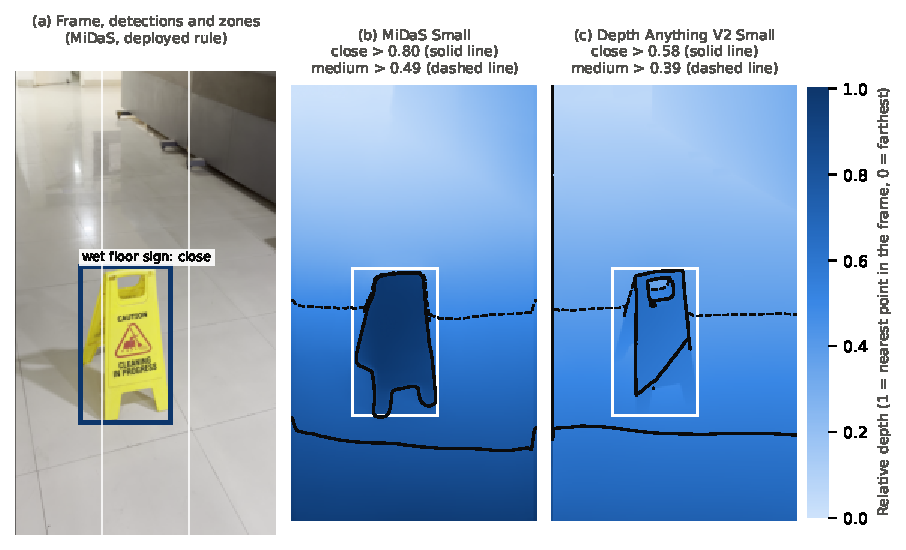
\includegraphics[width=0.45\textwidth]{relative_depth}
\caption{\rev{Relative depth as used by EchoPath} (sign.mp4, 2.0~s).
(a)~Detected box and zone. (b,~c)~Per-frame MiDaS Small and Depth Anything
V2 Small depth (1 = nearest point of this frame) with the frame's 75th
(solid, ``close'') and 50th (dashed, ``medium'') percentile contours. The
wet floor sign is close because its inner-box median lies above the 75th
percentile (0.98 for MiDaS); \rev{the values carry no metric scale.}}
\label{fig:reldepth}
\end{figure}

\subsection{End-to-end latency and frame rate}
\label{sec:latency}

Timings were measured on the RTX~4500 Ada workstation on every second frame
of the 13 videos (3,644 frames) after a 10-frame warm-up, with GPU work
synchronised before each timestamp (Table~\ref{tab:latency}). \rev{With MiDaS
Small and both models running, the pipeline processes 13.9 frames per
second.} \rev{Depth estimation is the largest stage because the depth map is
resized to the full $1080 \times 1920$ frame and copied to the CPU}; fusion
reaches 35~ms in cluttered frames, where two full-frame percentiles are
computed per box; HEVC decoding, which a live camera avoids, adds 11~ms.
For the end-to-end delay each video was streamed at its native
30~frames per second, the pipeline always processed the newest frame, and
alerts went through the speaker of Section~\ref{sec:audio} with its rate
limits (volume zero, which does not change the engine's timing); \rev{75 of 228
alerts were spoken and 153 dropped by the rate limits}, and the maxima were
212~ms to the alert decision and 5.6~s to speech. \rev{The sub-second delay
claimed originally therefore holds only in the median: a spoken alert lasts
2.3~s while the speaker accepts a new one every 1.5~s, so alerts queue}
(future work~(6)). \rev{The Jetson Nano has not been measured.}

\emph{Depth model selection.} \rev{MiDaS Small is retained. With equal alert
quality under the same rule (Section~\ref{sec:depth}), the choice rests on
cost}: (1)~a higher and steadier frame rate, with less than half the
95th-percentile frame time (Table~\ref{tab:latency}); \rev{(2)~size, 86 versus 99~MB
(originally given as 25 and 97~MB)}, or 92 versus 105~MB with YOLOv8n;
(3)~offline operation, which both support once their weights are cached (\rev{the
original claim that Depth Anything V2 needs an internet connection was
incorrect}); and (4)~dependencies, as MiDaS needs only PyTorch (with
timm) and Depth Anything V2 also Transformers. \rev{The higher alert
rate originally attributed to MiDaS came from the threshold rule.}

\begin{table}[!t]
\caption{\rev{Latency on the RTX~4500 Ada GPU with detection and depth estimation
running} (median / 95th percentile in ms). Offline rows time each of the
3,644 processed frames; the live replay streams the videos at 30~frames per
second and speaks the alerts through the deployed speaker.}
\label{tab:latency}
\footnotesize
\begin{tabular*}{\hsize}{@{\extracolsep{\fill}}lcc@{}}
\toprule
Stage & MiDaS Small (deployed) & Depth Anything V2 Small \\
\colrule
\multicolumn{3}{@{}l}{\emph{Offline, per processed frame}} \\
Frame decoding ($1080 \times 1920$ HEVC, CPU) & \rev{11 / 18} & \rev{12 / 14} \\
YOLOv8n detection / depth estimation & \rev{15 / 25 \;$\cdot$\; 46 / 65} & \rev{11 / 19 \;$\cdot$\; 51 / 132} \\
Fusion and alert decision & \rev{0.2 / 35} & \rev{0.2 / 103} \\
Pipeline per processed frame (frames per second) & \rev{71 / 109 (13.9)} & \rev{72 / 237 (10.7)} \\
\colrule
\multicolumn{3}{@{}l}{\emph{Live replay at 30 frames per second, with speech (MiDaS Small; 12.7 processed frames per second)}} \\
Frame capture to alert decision / to start of speech & \rev{85 / 137 \;$\cdot$\; 616 / 3,608} & -- \\
Wait in the speech queue / length of a spoken alert & \rev{455 / 3,426 \;$\cdot$\; 2,283 / 2,886} & -- \\
\botrule
\end{tabular*}
\end{table}

\section{Discussion}
\label{sec:discussion}

Evaluated without training near-duplicates, the revised model supports
EchoPath's design more credibly. Among the tier-1 hazards, v4 detects most
stairs and waste bins at the deployment threshold (Table~\ref{tab:perclass})
and all 43 wet floor signs, which, with this sample and a single source
dataset, must be confirmed in the target building before it can support a
safety claim. Missed stairs could cause a fall, so stairs recall is the most
important figure to improve. Chair (0.38 at confidence 0.25) and table remain
the weakest hazard classes, mainly in cluttered COCO scenes, followed by
person in crowded scenes, and fire\_extinguisher remains difficult,
consistent with work on small wall-mounted objects
indoors~\cite{farzaneh2022}; these classes need in-domain training data.
For a user, about three quarters of spoken alerts name a real nearby object,
but \rev{more than half of the obstacles in the walking path are not announced},
partly because of the rate limit and mainly because they are not detected,
and \rev{since the proximity zones are relative to each scene, ``close'' does not
guarantee a fixed safety margin}. Until missed hazards are much rarer,
EchoPath should be regarded as a supplement to the white cane, not a
replacement. \rev{Balancing reduces the spread among the tier-1 and tier-2
classes from more than 100:1 to about 4:1 per epoch}, but
notice\_board (48 training labels) and the synthetic water\_dispenser source
(115) remain small, and no training image comes from the target building.

Future work involves (1)~collecting and annotating images in the
Academic Block and other buildings, and annotating the 13 videos as an
in-domain test set; (2)~deployment on an NVIDIA Jetson Nano with a
chest-mounted camera as a wearable device; (3)~a user study with visually
impaired participants against a white-cane-only baseline, \rev{including
whether side obstacles should be announced}; (4)~larger YOLOv8 variants to
study the accuracy--latency trade-off on higher-compute platforms;
\rev{(5)~calibrating depth to metres against measured distances}, so that the
proximity zones correspond to distances; and (6)~fewer missed hazards,
through better detection of waste bins, water dispensers, unusual seating
and stairs in the target building and \rev{a speech queue that neither drops
newly appearing hazards nor delays them behind stale alerts}.

\section{Conclusion}
\label{sec:conclusion}

EchoPath is an infrastructure-free, YOLOv8n-based object detection and audio
navigation system for visually impaired people in indoor academic buildings.
A data audit (attributed sources, no leakage, completed labels,
importance-weighted balancing) raises the mean mAP@50 on identical
leakage-free images from 0.608 to 0.813. The pipeline runs at 13.9 frames
per second on a workstation GPU with a median delay of 0.62~s to speech, the
two depth models give alerts of the same quality under identical rules, and
YOLOv8n~\cite{jocher2023yolov8} is ten times smaller and 3.7 times faster
than RT-DETR-L~\cite{zhao2023rtdetr}. Three quarters of spoken alerts are
correct, but more than half of the in-path obstacles are missed, mainly by
the detector, so detection in the target building is the next priority. Students with visual impairments in Indian institutions represent a
real and largely unmet need~\cite{at2030}; existing tools require
infrastructure investment~\cite{ahmetovic2016navcog} or lack real-time
directional guidance~\cite{messaoudi2022}, and EchoPath's
infrastructure-free design offers them an improved means of navigating
campus buildings independently.

\section*{Acknowledgements}

The authors thank the Department of Artificial Intelligence and Data Science,
Gati Shakti Vishwavidyalaya, for providing the computing resources used in this
work.

\begin{thebibliography}{00}

%% References follow the Procedia (Elsevier numbered/Vancouver) style:
%% journal abbreviations, Year;Vol(Issue):pages, "In: ...; Year, p. x--y."
%% for proceedings, and "Title, Repository, vN; Year." for datasets.
\bibitem{who2023}
World Health Organization. Blindness and vision impairment [fact sheet],
\url{https://www.who.int/news-room/fact-sheets/detail/blindness-and-visual-impairment};
2023 [accessed 23 October 2026].

\bibitem{singh2022}
Mannava S, Borah RR, Shamanna BR. Current estimates of the economic burden
of blindness and visual impairment in India: a cost of illness study. Indian
J Ophthalmol 2022;70(6):2141--5.

\bibitem{aishe2021}
Ministry of Education, Government of India. All India Survey on Higher
Education 2021--22. New Delhi: Department of Higher Education; 2024.
\url{https://aishe.gov.in/document/aishe-final-report-2021-22/}

\bibitem{aishe2019}
Ministry of Education, Government of India. All India Survey on Higher
Education 2019--20. New Delhi: Department of Higher Education; 2021.
\url{https://aishe.gov.in/document/aishe-final-report-2019-20/}

\bibitem{aishe_impaired_data}
An analytical report on the availability of government data for visually
impaired students in India. Scribd,
\url{https://www.scribd.com/document/905928671/Blind-Students-Data-India-1};
n.d. [accessed 23 October 2026].

\bibitem{at2030}
Bhatnagar T, Upadhyay V, Rao PVM, Marquardt N, Miodownik M, Holloway C.
Brilliance and resilience: a new perspective to the challenges, practices and
needs of university students with visual impairments in India. In:
Human-Computer Interaction -- INTERACT 2023. Lecture Notes in Computer
Science, vol 14142. Cham: Springer; 2023, p. 67--88.

\bibitem{abdul2023}
Abdullah, Waheed A. Opportunities and barriers to disabled students in
higher education: an explorative study of visually impaired students of
Aligarh Muslim University, India. Mediterr J Soc Sci 2023;14(1):78--87.

\bibitem{redmon2016yolo}
Redmon J, Divvala S, Girshick R, Farhadi A. You only look once: unified,
real-time object detection. In: Proceedings of the IEEE Conference on
Computer Vision and Pattern Recognition (CVPR); 2016, p. 779--88.

\bibitem{jocher2023yolov8}
Jocher G, Chaurasia A, Qiu J. Ultralytics YOLOv8 (Version 8.0.0). GitHub;
2023. \url{https://github.com/ultralytics/ultralytics}

\bibitem{zhao2023rtdetr}
Zhao Y, Lv W, Xu S, Wei J, Wang G, Dang Q, et al. DETRs beat YOLOs on
real-time object detection. arXiv preprint arXiv:2304.08069; 2023.

\bibitem{bhatlawande2014}
Bhatlawande S, Mahadevappa M, Mukherjee J, Biswas M, Das D, Gupta S. Design,
development, and clinical evaluation of the electronic mobility cane for
vision rehabilitation. IEEE Trans Neural Syst Rehabil Eng
2014;22(6):1148--59.

\bibitem{li2020yolo}
Okolo GI, Althobaiti T, Ramzan N. Smart assistive navigation system for
visually impaired people. J Disabil Res 2025;4(1):20240086.
\url{https://doi.org/10.57197/JDR-2024-0086}

\bibitem{ranftl2020midas}
Ranftl R, Lasinger K, Hafner D, Schindler K, Koltun V. Towards robust
monocular depth estimation: mixing datasets for zero-shot cross-dataset
transfer. IEEE Trans Pattern Anal Mach Intell 2022;44(3):1623--37.

\bibitem{ahmetovic2016navcog}
Ahmetovic D, Gleason C, Ruan C, Kitani K, Takagi H, Asakawa C. NavCog: a
navigational cognitive assistant for the blind. In: Proceedings of the 18th
International Conference on Human-Computer Interaction with Mobile Devices
and Services (MobileHCI); 2016, p. 90--9.

\bibitem{ahmetovic2019sonification}
Ahmetovic D, Avanzini F, Barat\`{e} A, Bernareggi C, Galimberti G, Ludovico
LA, et al. Sonification of rotation instructions to support navigation of
people with visual impairment. In: Proceedings of the IEEE International
Conference on Pervasive Computing and Communications (PerCom); 2019, p. 1--10.

\bibitem{messaoudi2022}
Messaoudi MD, Menelas BAJ, Mcheick H. Review of navigation assistive tools
and technologies for the visually impaired. Sensors 2022;22(20):7888.
\url{https://doi.org/10.3390/s22207888}

\bibitem{yu2025visa}
Yu X, Saniie J. Visual impairment spatial awareness system for indoor
navigation and daily activities. J Imaging 2025;11(1):9.
\url{https://doi.org/10.3390/jimaging11010009}

\bibitem{kedia2017mavi}
Kedia R, Yoosuf KK, Dedeepya P, Fazal M, Arora C, Balakrishnan M. MAVI: an
embedded device to assist mobility of visually impaired. In: Proceedings of
the 30th International Conference on VLSI Design (VLSID); 2017, p. 213--8.

\bibitem{kasture2021}
Kasture P, Tangade A, Pole A, Kumkar A, Jagtap Y. Real-time object detection
using YOLO algorithm for blind people. Int J Adv Res Sci Commun Technol
2021;5(2):152--6.

\bibitem{sharma2020}
Sharma T, Bali S, Yadav S. Obstacle detection system for visually impaired
person. Int Res J Eng Technol 2020;7(9):1951--3.

\bibitem{lin2014coco}
Lin TY, Maire M, Belongie S, Hays J, Perona P, Ramanan D, et al. Microsoft
COCO: common objects in context. In: Proceedings of the European Conference
on Computer Vision (ECCV); 2014, p. 740--55.

%% ---- Training datasets (Roboflow Universe, all CC BY 4.0) -------------------
\bibitem{rf_person}
Riga R. person, Roboflow Universe, v4; 2024. CC BY 4.0. \href{https://universe.roboflow.com/rasheed-riga-ilxzv/person-fjw64}{\nolinkurl{universe.roboflow.com/rasheed-riga-ilxzv/person-fjw64}}

\bibitem{rf_chair}
Object Detect. chairs, Roboflow Universe, v5; 2025. CC BY 4.0. \href{https://universe.roboflow.com/object-detect-zjtnj/chairs-dnhsd}{\nolinkurl{universe.roboflow.com/object-detect-zjtnj/chairs-dnhsd}}

\bibitem{rf_door}
Nyla. Door, Roboflow Universe, v1; 2021. CC BY 4.0. \href{https://universe.roboflow.com/nyla/door-ex6s8}{\nolinkurl{universe.roboflow.com/nyla/door-ex6s8}}

\bibitem{rf_navigation}
Dataset. Navigation, Roboflow Universe, v1; 2025. CC BY 4.0. \href{https://universe.roboflow.com/dataset-kenli/navigation-hlzh2}{\nolinkurl{universe.roboflow.com/dataset-kenli/navigation-hlzh2}}

\bibitem{rf_whiteboard}
Student. White-board Detection, Roboflow Universe, v2--4; 2024. CC BY 4.0. \href{https://universe.roboflow.com/student-cbw0s/white-board-detection}{\nolinkurl{universe.roboflow.com/student-cbw0s/white-board-detection}}

\bibitem{rf_notice}
Library. Notice boards iiee, Roboflow Universe, v1--3; 2025. CC BY 4.0. \href{https://universe.roboflow.com/library-nbtst/notice-boards-iiee-ydmbd}{\nolinkurl{universe.roboflow.com/library-nbtst/notice-boards-iiee-ydmbd}}

\bibitem{rf_elevatordoor}
Elevator Panel detection. elevator\_door, Roboflow Universe, v15; 2026. CC BY 4.0. \href{https://universe.roboflow.com/elevator-panel-detection/elevator_door-riuxl}{\nolinkurl{universe.roboflow.com/elevator-panel-detection/elevator_door-riuxl}}

\bibitem{rf_column}
SD. Column, Roboflow Universe, v2; 2025. CC BY 4.0. \href{https://universe.roboflow.com/sd-ug5qc/column-2i5mg}{\nolinkurl{universe.roboflow.com/sd-ug5qc/column-2i5mg}}

\bibitem{rf_window}
rkdf. windows, Roboflow Universe, v1; 2024. CC BY 4.0. \href{https://universe.roboflow.com/rkdf/windows-qvnbq}{\nolinkurl{universe.roboflow.com/rkdf/windows-qvnbq}}

\bibitem{rf_water}
akaike. Water dispenser, Roboflow Universe, v1; 2022. CC BY 4.0. \href{https://universe.roboflow.com/akaike/water-dispenser}{\nolinkurl{universe.roboflow.com/akaike/water-dispenser}}

\bibitem{rf_plant}
Manans Workspace. Plant Object Detection, Roboflow Universe, v4; 2025. CC BY 4.0. \href{https://universe.roboflow.com/manans-workspace/plant-object-detection}{\nolinkurl{universe.roboflow.com/manans-workspace/plant-object-detection}}

\bibitem{rf_wastebin}
Khan U. waste-bin, Roboflow Universe, v1--2; 2022. CC BY 4.0. \href{https://universe.roboflow.com/umer-khan/waste-bin}{\nolinkurl{universe.roboflow.com/umer-khan/waste-bin}}

\bibitem{rf_dustbin}
Workspace. Dustbin Detection, Roboflow Universe, v1; 2025. CC BY 4.0. \href{https://universe.roboflow.com/workspace-yus7k/dustbin-detection-u76yd}{\nolinkurl{universe.roboflow.com/workspace-yus7k/dustbin-detection-u76yd}}

\bibitem{rf_trashbin}
trialyolo. Trash\_bin\_detection, Roboflow Universe, v1; 2025. CC BY 4.0. \href{https://universe.roboflow.com/trialyolo/trash_bin_detection-9glxi}{\nolinkurl{universe.roboflow.com/trialyolo/trash_bin_detection-9glxi}}

\bibitem{rf_fire}
Kieran. Fire Extinguisher, Roboflow Universe, v2; 2023. CC BY 4.0. \href{https://universe.roboflow.com/kieran-xejdv/fire-extinguisher-ftnny}{\nolinkurl{universe.roboflow.com/kieran-xejdv/fire-extinguisher-ftnny}}

\bibitem{rf_wetfloor}
FRC 5881. wet floor, Roboflow Universe, v1; 2024. CC BY 4.0. \href{https://universe.roboflow.com/frc-5881/wet-floor-nhjwl}{\nolinkurl{universe.roboflow.com/frc-5881/wet-floor-nhjwl}}

\bibitem{rf_table}
AIfull. table-person, Roboflow Universe, v8--9; 2024. CC BY 4.0. \href{https://universe.roboflow.com/aifull/table-person}{\nolinkurl{universe.roboflow.com/aifull/table-person}}

\bibitem{rf_monitor}
Object detection. Computer monitor, Roboflow Universe, v1; 2023. CC BY 4.0. \href{https://universe.roboflow.com/object-detection-bwxix/computer-monitor}{\nolinkurl{universe.roboflow.com/object-detection-bwxix/computer-monitor}}

%% ---- Cited after the training datasets --------------------------------------
\bibitem{depthanythingv2}
Yang L, Kang B, Huang Z, Zhao Z, Xu X, Feng J, et al. Depth Anything V2.
arXiv preprint arXiv:2406.09414; 2024.

\bibitem{farzaneh2022}
Farzaneh MJ, Mohammadi HM. Implementation of a blind navigation method in
outdoors/indoors areas. arXiv preprint arXiv:2212.12185; 2022.

\end{thebibliography}

\end{document}
